\documentclass[Interploate_hadwritten_Digits.tex]{subfiles}

\begin{document}
	\subsection{Histograme Leistung}
	\begin{multicols}{2}
		\begin{Figure}
			\centering
			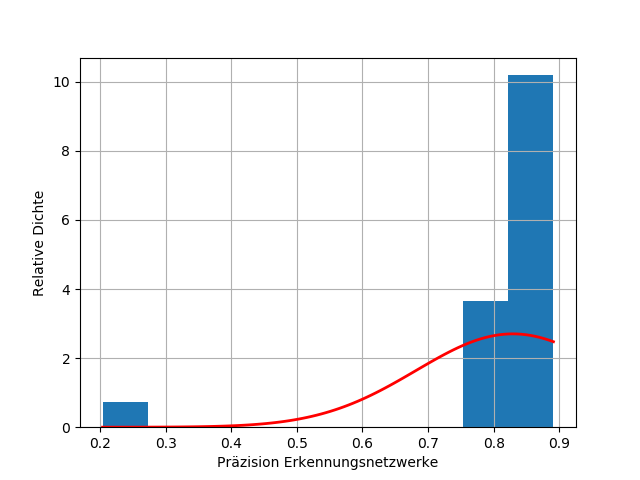
\includegraphics[width=\linewidth]{img/results/histogram_network_accuracy.png}
			\captionof{figure}{Präzision der Klassifizierungsnetze}
		\end{Figure}
		\begin{Figure}
			\centering
			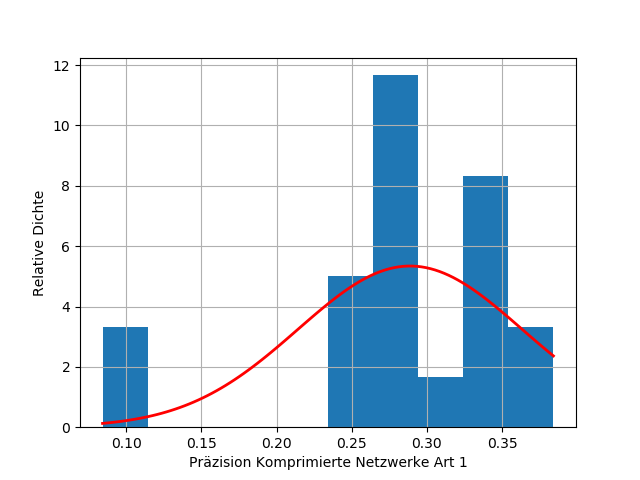
\includegraphics[width=\linewidth]{img/results/histogram_compressed_network_accuracy.png}
			\captionof{figure}{Präzision mit Komprimierung Art 1}
		\end{Figure}
		\begin{Figure}
			\centering
			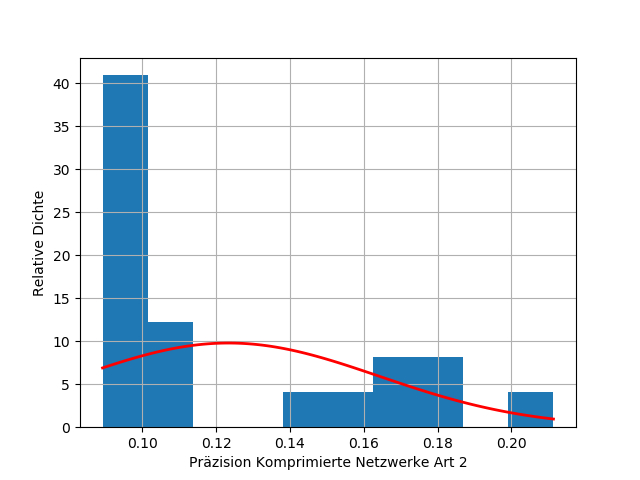
\includegraphics[width=\linewidth]{img/results/histogram_compressed_network_v2_accuracy.png}
			\captionof{figure}{Präzision mit Komprimierung Art 2}
		\end{Figure}
		\begin{Figure}
			\centering
			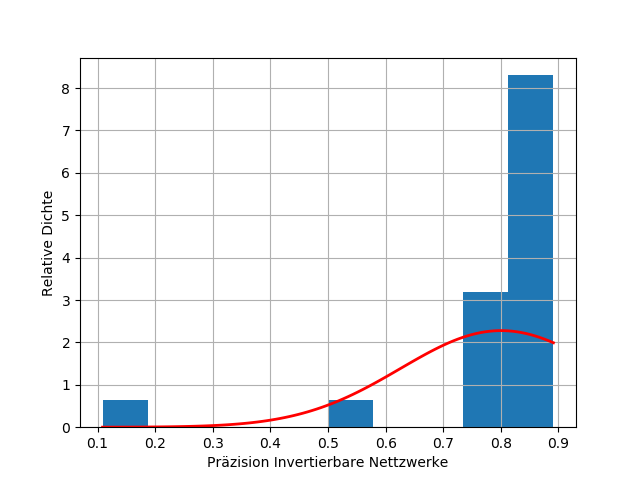
\includegraphics[width=\linewidth]{img/results/histogram_inverted_network_accuracy.png}
			\captionof{figure}{Präzision Invertierbares Netz}
		\end{Figure}
		\begin{Figure}
			\centering
			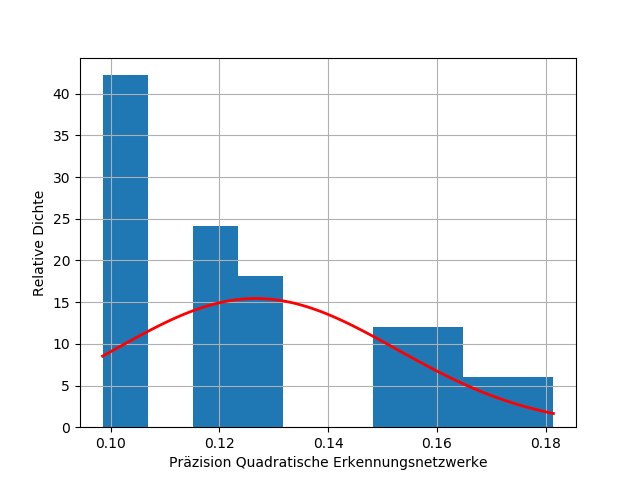
\includegraphics[width=\linewidth]{img/results/histogram_squared_network_accuracy.png}
			\captionof{figure}{Präzision Kassifikation Quadratische Matrizen}
		\end{Figure}
		\begin{Figure}
			\centering
			\includegraphics[width=\linewidth]{img/results/histogram_squared_inverted_network_accuracy.png}
			\captionof{figure}{Präzision Invertierung Quadratische Matrizen}
		\end{Figure}
	\end{multicols}
	\newpage
	
	\subsection{Konfusionsmartizen}
	\label{sec:apendix_konfusion_network}
	
	\subsubsection{Klassifizierungs Netz}
	\foreach \n in {0, ..., 19} {\subfile{img/results/confusion_table_network_\n}}
	
	\subsubsection{Komprimierung Version 1}
	\begin{multicols}{2}
		\foreach \n in {0, ..., 19} {\subfile{img/results/confusion_table_compressed_network_\n}}
	\end{multicols}
	
	\subsubsection{Komprimierung Version 2}
	\foreach \n in {0, ..., 19} {\subfile{img/results/confusion_table_compressed_network_v2_\n}}
	
	\subsubsection{Invertierbares Netz}
	\foreach \n in {0, ..., 19} {\subfile{img/results/confusion_table_inverted_network_\n}}
	
	\subsubsection{Klassifizierung Quadratische Netze}
	\begin{multicols}{2}
		\foreach \n in {0, ..., 19} {\subfile{img/results/confusion_table_squared_network_\n}}
	\end{multicols}
	
	\subsubsection{Invertierung Quadratische Netze}
	\begin{multicols}{2}
		\foreach \n in {0, ..., 19} {\subfile{img/results/confusion_table_squared_inverted_network_\n}}
	\end{multicols}
	\newpage
	
	\subsection{Fehler Invertierung}
	\begin{multicols}{2}
		\begin{Figure}
			\centering
			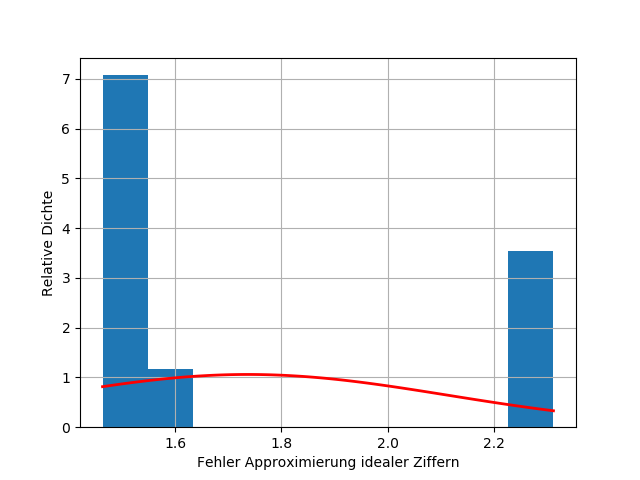
\includegraphics[width=\linewidth]{img/results/histogram_approximation_error_ideal.png}
			\captionof{figure}{Fehler Approximierung idealer Ziffern}
		\end{Figure}
		\begin{Figure}
			\centering
			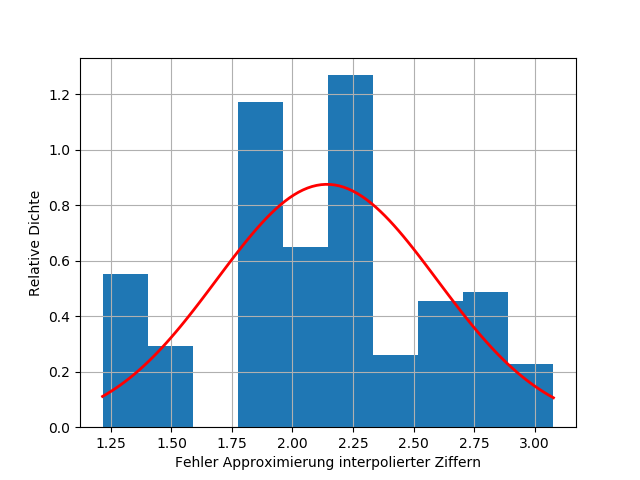
\includegraphics[width=\linewidth]{img/results/histogram_approximation_error_interpolation.png}
			\captionof{figure}{Fehler Approximierung interploierter Ziffern}
		\end{Figure}
	\end{multicols}
	
	\subsection{Bilder aus der Invertierung}
	\label{sec:apendix_numbers_inversion}
	\subsubsection{Ideale Ziffern}
	\begin{tabular}{cccc}
		Ziffer & Invertierung & Quadratische Invertierung & Approximation \\
		0 & 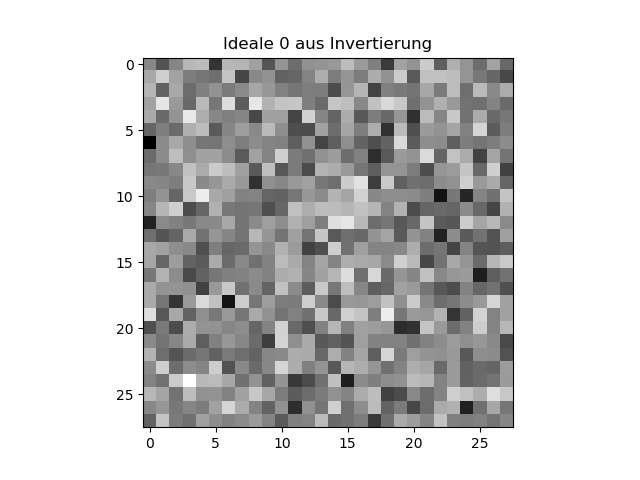
\includegraphics[scale=0.3]{img/results/ideal_0_inverted.png} & \includegraphics[scale=0.3]{img/results/ideal_0_squared_inverted.png} & \includegraphics[scale=0.3]{img/results/ideal_0_approximated.png} \\
		1 & \includegraphics[scale=0.3]{img/results/ideal_1_inverted.png} & \includegraphics[scale=0.3]{img/results/ideal_1_squared_inverted.png} & \includegraphics[scale=0.3]{img/results/ideal_1_approximated.png} \\
		2 & \includegraphics[scale=0.3]{img/results/ideal_2_inverted.png} & \includegraphics[scale=0.3]{img/results/ideal_2_squared_inverted.png} & \includegraphics[scale=0.3]{img/results/ideal_2_approximated.png} \\
		3 & \includegraphics[scale=0.3]{img/results/ideal_3_inverted.png} & \includegraphics[scale=0.3]{img/results/ideal_3_squared_inverted.png} & \includegraphics[scale=0.3]{img/results/ideal_3_approximated.png} \\
		4 & \includegraphics[scale=0.3]{img/results/ideal_4_inverted.png} & \includegraphics[scale=0.3]{img/results/ideal_4_squared_inverted.png} & \includegraphics[scale=0.3]{img/results/ideal_4_approximated.png} \\
		5 & \includegraphics[scale=0.3]{img/results/ideal_5_inverted.png} & \includegraphics[scale=0.3]{img/results/ideal_5_squared_inverted.png} & \includegraphics[scale=0.3]{img/results/ideal_5_approximated.png} \\
	\end{tabular}
	\begin{tabular}{cccc}
		Ziffer & Invertierung & Quadratische Invertierung & Approximation \\
		6 & \includegraphics[scale=0.3]{img/results/ideal_6_inverted.png} & \includegraphics[scale=0.3]{img/results/ideal_6_squared_inverted.png} & \includegraphics[scale=0.3]{img/results/ideal_6_approximated.png} \\
		7 & \includegraphics[scale=0.3]{img/results/ideal_7_inverted.png} & \includegraphics[scale=0.3]{img/results/ideal_7_squared_inverted.png} & 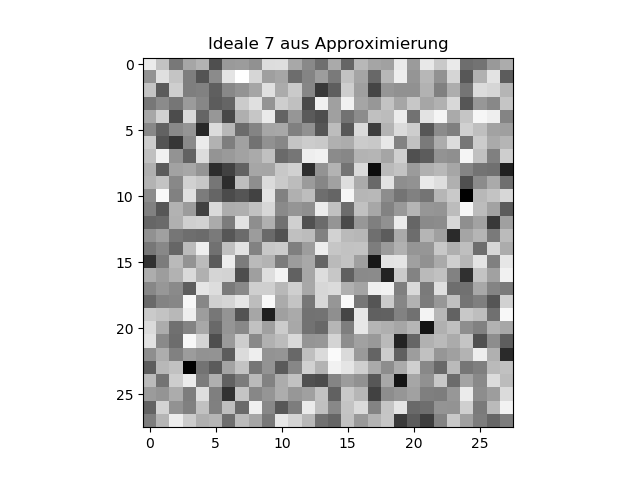
\includegraphics[scale=0.3]{img/results/ideal_7_approximated.png} \\
		8 & \includegraphics[scale=0.3]{img/results/ideal_8_inverted.png} & \includegraphics[scale=0.3]{img/results/ideal_8_squared_inverted.png} & \includegraphics[scale=0.3]{img/results/ideal_8_approximated.png} \\
		9 & \includegraphics[scale=0.3]{img/results/ideal_9_inverted.png} & \includegraphics[scale=0.3]{img/results/ideal_9_squared_inverted.png} & \includegraphics[scale=0.3]{img/results/ideal_9_approximated.png} \\
	\end{tabular}
		
	\subsubsection{Interpolierte Ziffern}
	\begin{tabular}{cccc}
		Interpolation & Invertierung & Quadratische Invertierung & Approximation \\
		0 -> 1: 25 \% & \includegraphics[scale=0.25]{img/results/interpolated_0_1_25_inverted.png} & \includegraphics[scale=0.25]{img/results/interpolated_0_1_25_squared_inverted.png} & \includegraphics[scale=0.25]{img/results/interpolated_0_1_25_approximated.png} \\
		0 -> 1: 50 \% & \includegraphics[scale=0.25]{img/results/interpolated_0_1_50_inverted.png} & \includegraphics[scale=0.25]{img/results/interpolated_0_1_50_squared_inverted.png} & \includegraphics[scale=0.25]{img/results/interpolated_0_1_50_approximated.png} \\
		0 -> 1: 75 \% & \includegraphics[scale=0.25]{img/results/interpolated_0_1_75_inverted.png} & \includegraphics[scale=0.25]{img/results/interpolated_0_1_75_squared_inverted.png} & \includegraphics[scale=0.25]{img/results/interpolated_0_1_75_approximated.png} \\
		0 -> 2: 25 \% & \includegraphics[scale=0.25]{img/results/interpolated_0_2_25_inverted.png} & \includegraphics[scale=0.25]{img/results/interpolated_0_2_25_squared_inverted.png} & \includegraphics[scale=0.25]{img/results/interpolated_0_2_25_approximated.png} \\
		0 -> 2: 50 \% & \includegraphics[scale=0.25]{img/results/interpolated_0_2_50_inverted.png} & \includegraphics[scale=0.25]{img/results/interpolated_0_2_50_squared_inverted.png} & \includegraphics[scale=0.25]{img/results/interpolated_0_2_50_approximated.png} \\
		0 -> 2: 75 \% & \includegraphics[scale=0.25]{img/results/interpolated_0_2_75_inverted.png} & \includegraphics[scale=0.25]{img/results/interpolated_0_2_75_squared_inverted.png} & \includegraphics[scale=0.25]{img/results/interpolated_0_2_75_approximated.png} \\
		0 -> 3: 25 \% & \includegraphics[scale=0.25]{img/results/interpolated_0_3_25_inverted.png} & \includegraphics[scale=0.25]{img/results/interpolated_0_3_25_squared_inverted.png} & \includegraphics[scale=0.25]{img/results/interpolated_0_3_25_approximated.png} \\
	\end{tabular}
	\newpage
	\begin{tabular}{cccc}
		Interpolation & Invertierung & Quadratische Invertierung & Approximation \\
		0 -> 3: 50 \% & \includegraphics[scale=0.25]{img/results/interpolated_0_3_50_inverted.png} & \includegraphics[scale=0.25]{img/results/interpolated_0_3_50_squared_inverted.png} & \includegraphics[scale=0.25]{img/results/interpolated_0_3_50_approximated.png} \\
		0 -> 3: 75 \% & \includegraphics[scale=0.25]{img/results/interpolated_0_3_75_inverted.png} & \includegraphics[scale=0.25]{img/results/interpolated_0_3_75_squared_inverted.png} & \includegraphics[scale=0.25]{img/results/interpolated_0_3_75_approximated.png} \\
		0 -> 4: 25 \% & \includegraphics[scale=0.25]{img/results/interpolated_0_4_25_inverted.png} & \includegraphics[scale=0.25]{img/results/interpolated_0_4_25_squared_inverted.png} & \includegraphics[scale=0.25]{img/results/interpolated_0_4_25_approximated.png} \\
		0 -> 4: 50 \% & \includegraphics[scale=0.25]{img/results/interpolated_0_4_50_inverted.png} & \includegraphics[scale=0.25]{img/results/interpolated_0_4_50_squared_inverted.png} & \includegraphics[scale=0.25]{img/results/interpolated_0_4_50_approximated.png} \\
		0 -> 4: 75 \% & \includegraphics[scale=0.25]{img/results/interpolated_0_4_75_inverted.png} & \includegraphics[scale=0.25]{img/results/interpolated_0_4_75_squared_inverted.png} & \includegraphics[scale=0.25]{img/results/interpolated_0_4_75_approximated.png} \\
		0 -> 5: 25 \% & \includegraphics[scale=0.25]{img/results/interpolated_0_5_25_inverted.png} & \includegraphics[scale=0.25]{img/results/interpolated_0_5_25_squared_inverted.png} & \includegraphics[scale=0.25]{img/results/interpolated_0_5_25_approximated.png} \\
		0 -> 5: 50 \% & \includegraphics[scale=0.25]{img/results/interpolated_0_5_50_inverted.png} & \includegraphics[scale=0.25]{img/results/interpolated_0_5_50_squared_inverted.png} & \includegraphics[scale=0.25]{img/results/interpolated_0_5_50_approximated.png} \\
	\end{tabular}
	\newpage
	\begin{tabular}{cccc}
		Interpolation & Invertierung & Quadratische Invertierung & Approximation \\
		0 -> 5: 75 \% & \includegraphics[scale=0.25]{img/results/interpolated_0_5_75_inverted.png} & \includegraphics[scale=0.25]{img/results/interpolated_0_5_75_squared_inverted.png} & \includegraphics[scale=0.25]{img/results/interpolated_0_5_75_approximated.png} \\
		0 -> 6: 25 \% & \includegraphics[scale=0.25]{img/results/interpolated_0_6_25_inverted.png} & \includegraphics[scale=0.25]{img/results/interpolated_0_6_25_squared_inverted.png} & \includegraphics[scale=0.25]{img/results/interpolated_0_6_25_approximated.png} \\
		0 -> 6: 50 \% & \includegraphics[scale=0.25]{img/results/interpolated_0_6_50_inverted.png} & \includegraphics[scale=0.25]{img/results/interpolated_0_6_50_squared_inverted.png} & \includegraphics[scale=0.25]{img/results/interpolated_0_6_50_approximated.png} \\
		0 -> 6: 75 \% & \includegraphics[scale=0.25]{img/results/interpolated_0_6_75_inverted.png} & \includegraphics[scale=0.25]{img/results/interpolated_0_6_75_squared_inverted.png} & \includegraphics[scale=0.25]{img/results/interpolated_0_6_75_approximated.png} \\
		0 -> 7: 25 \% & \includegraphics[scale=0.25]{img/results/interpolated_0_7_25_inverted.png} & \includegraphics[scale=0.25]{img/results/interpolated_0_7_25_squared_inverted.png} & \includegraphics[scale=0.25]{img/results/interpolated_0_7_25_approximated.png} \\
		0 -> 7: 50 \% & \includegraphics[scale=0.25]{img/results/interpolated_0_7_50_inverted.png} & \includegraphics[scale=0.25]{img/results/interpolated_0_7_50_squared_inverted.png} & \includegraphics[scale=0.25]{img/results/interpolated_0_7_50_approximated.png} \\
		0 -> 7: 75 \% & \includegraphics[scale=0.25]{img/results/interpolated_0_7_75_inverted.png} & \includegraphics[scale=0.25]{img/results/interpolated_0_7_75_squared_inverted.png} & \includegraphics[scale=0.25]{img/results/interpolated_0_7_75_approximated.png} \\
	\end{tabular}
	\newpage
	\begin{tabular}{cccc}
		Interpolation & Invertierung & Quadratische Invertierung & Approximation \\
		0 -> 8: 25 \% & \includegraphics[scale=0.25]{img/results/interpolated_0_8_25_inverted.png} & \includegraphics[scale=0.25]{img/results/interpolated_0_8_25_squared_inverted.png} & \includegraphics[scale=0.25]{img/results/interpolated_0_8_25_approximated.png} \\
		0 -> 8: 50 \% & \includegraphics[scale=0.25]{img/results/interpolated_0_8_50_inverted.png} & \includegraphics[scale=0.25]{img/results/interpolated_0_8_50_squared_inverted.png} & \includegraphics[scale=0.25]{img/results/interpolated_0_8_50_approximated.png} \\
		0 -> 8: 75 \% & \includegraphics[scale=0.25]{img/results/interpolated_0_8_75_inverted.png} & \includegraphics[scale=0.25]{img/results/interpolated_0_8_75_squared_inverted.png} & \includegraphics[scale=0.25]{img/results/interpolated_0_8_75_approximated.png} \\
		0 -> 9: 25 \% & \includegraphics[scale=0.25]{img/results/interpolated_0_9_25_inverted.png} & \includegraphics[scale=0.25]{img/results/interpolated_0_9_25_squared_inverted.png} & \includegraphics[scale=0.25]{img/results/interpolated_0_9_25_approximated.png} \\
		0 -> 9: 50 \% & \includegraphics[scale=0.25]{img/results/interpolated_0_9_50_inverted.png} & \includegraphics[scale=0.25]{img/results/interpolated_0_9_50_squared_inverted.png} & \includegraphics[scale=0.25]{img/results/interpolated_0_9_50_approximated.png} \\
		0 -> 9: 75 \% & \includegraphics[scale=0.25]{img/results/interpolated_0_9_75_inverted.png} & \includegraphics[scale=0.25]{img/results/interpolated_0_9_75_squared_inverted.png} & \includegraphics[scale=0.25]{img/results/interpolated_0_9_75_approximated.png} \\
		1 -> 2: 25 \% & \includegraphics[scale=0.25]{img/results/interpolated_1_2_25_inverted.png} & \includegraphics[scale=0.25]{img/results/interpolated_1_2_25_squared_inverted.png} & \includegraphics[scale=0.25]{img/results/interpolated_1_2_25_approximated.png} \\
	\end{tabular}
	\newpage
	\begin{tabular}{cccc}
		Interpolation & Invertierung & Quadratische Invertierung & Approximation \\
		1 -> 2: 50 \% & \includegraphics[scale=0.25]{img/results/interpolated_1_2_50_inverted.png} & \includegraphics[scale=0.25]{img/results/interpolated_1_2_50_squared_inverted.png} & \includegraphics[scale=0.25]{img/results/interpolated_1_2_50_approximated.png} \\
		1 -> 2: 75 \% & \includegraphics[scale=0.25]{img/results/interpolated_1_2_75_inverted.png} & \includegraphics[scale=0.25]{img/results/interpolated_1_2_75_squared_inverted.png} & \includegraphics[scale=0.25]{img/results/interpolated_1_2_75_approximated.png} \\
		1 -> 3: 25 \% & \includegraphics[scale=0.25]{img/results/interpolated_1_3_25_inverted.png} & \includegraphics[scale=0.25]{img/results/interpolated_1_3_25_squared_inverted.png} & \includegraphics[scale=0.25]{img/results/interpolated_1_3_25_approximated.png} \\
		1 -> 3: 50 \% & \includegraphics[scale=0.25]{img/results/interpolated_1_3_50_inverted.png} & \includegraphics[scale=0.25]{img/results/interpolated_1_3_50_squared_inverted.png} & \includegraphics[scale=0.25]{img/results/interpolated_1_3_50_approximated.png} \\
		1 -> 3: 75 \% & \includegraphics[scale=0.25]{img/results/interpolated_1_3_75_inverted.png} & \includegraphics[scale=0.25]{img/results/interpolated_1_3_75_squared_inverted.png} & \includegraphics[scale=0.25]{img/results/interpolated_1_3_75_approximated.png} \\
		1 -> 4: 25 \% & \includegraphics[scale=0.25]{img/results/interpolated_1_4_25_inverted.png} & \includegraphics[scale=0.25]{img/results/interpolated_1_4_25_squared_inverted.png} & \includegraphics[scale=0.25]{img/results/interpolated_1_4_25_approximated.png} \\
		1 -> 4: 50 \% & \includegraphics[scale=0.25]{img/results/interpolated_1_4_50_inverted.png} & \includegraphics[scale=0.25]{img/results/interpolated_1_4_50_squared_inverted.png} & \includegraphics[scale=0.25]{img/results/interpolated_1_4_50_approximated.png} \\
	\end{tabular}
	\newpage
	\begin{tabular}{cccc}
		Interpolation & Invertierung & Quadratische Invertierung & Approximation \\
		1 -> 4: 75 \% & \includegraphics[scale=0.25]{img/results/interpolated_1_4_75_inverted.png} & \includegraphics[scale=0.25]{img/results/interpolated_1_4_75_squared_inverted.png} & \includegraphics[scale=0.25]{img/results/interpolated_1_4_75_approximated.png} \\
		1 -> 5: 25 \% & \includegraphics[scale=0.25]{img/results/interpolated_1_5_25_inverted.png} & \includegraphics[scale=0.25]{img/results/interpolated_1_5_25_squared_inverted.png} & \includegraphics[scale=0.25]{img/results/interpolated_1_5_25_approximated.png} \\
		1 -> 5: 50 \% & \includegraphics[scale=0.25]{img/results/interpolated_1_5_50_inverted.png} & \includegraphics[scale=0.25]{img/results/interpolated_1_5_50_squared_inverted.png} & \includegraphics[scale=0.25]{img/results/interpolated_1_5_50_approximated.png} \\
		1 -> 5: 75 \% & \includegraphics[scale=0.25]{img/results/interpolated_1_5_75_inverted.png} & \includegraphics[scale=0.25]{img/results/interpolated_1_5_75_squared_inverted.png} & \includegraphics[scale=0.25]{img/results/interpolated_1_5_75_approximated.png} \\
		1 -> 6: 25 \% & \includegraphics[scale=0.25]{img/results/interpolated_1_6_25_inverted.png} & \includegraphics[scale=0.25]{img/results/interpolated_1_6_25_squared_inverted.png} & \includegraphics[scale=0.25]{img/results/interpolated_1_6_25_approximated.png} \\
		1 -> 6: 50 \% & \includegraphics[scale=0.25]{img/results/interpolated_1_6_50_inverted.png} & \includegraphics[scale=0.25]{img/results/interpolated_1_6_50_squared_inverted.png} & \includegraphics[scale=0.25]{img/results/interpolated_1_6_50_approximated.png} \\
		1 -> 6: 75 \% & \includegraphics[scale=0.25]{img/results/interpolated_1_6_75_inverted.png} & \includegraphics[scale=0.25]{img/results/interpolated_1_6_75_squared_inverted.png} & \includegraphics[scale=0.25]{img/results/interpolated_1_6_75_approximated.png} \\
	\end{tabular}
	\newpage
	\begin{tabular}{cccc}
		Interpolation & Invertierung & Quadratische Invertierung & Approximation \\
		1 -> 7: 25 \% & \includegraphics[scale=0.25]{img/results/interpolated_1_7_25_inverted.png} & \includegraphics[scale=0.25]{img/results/interpolated_1_7_25_squared_inverted.png} & \includegraphics[scale=0.25]{img/results/interpolated_1_7_25_approximated.png} \\
		1 -> 7: 50 \% & \includegraphics[scale=0.25]{img/results/interpolated_1_7_50_inverted.png} & \includegraphics[scale=0.25]{img/results/interpolated_1_7_50_squared_inverted.png} & \includegraphics[scale=0.25]{img/results/interpolated_1_7_50_approximated.png} \\
		1 -> 7: 75 \% & \includegraphics[scale=0.25]{img/results/interpolated_1_7_75_inverted.png} & \includegraphics[scale=0.25]{img/results/interpolated_1_7_75_squared_inverted.png} & \includegraphics[scale=0.25]{img/results/interpolated_1_7_75_approximated.png} \\
		1 -> 8: 25 \% & \includegraphics[scale=0.25]{img/results/interpolated_1_8_25_inverted.png} & \includegraphics[scale=0.25]{img/results/interpolated_1_8_25_squared_inverted.png} & \includegraphics[scale=0.25]{img/results/interpolated_1_8_25_approximated.png} \\
		1 -> 8: 50 \% & \includegraphics[scale=0.25]{img/results/interpolated_1_8_50_inverted.png} & \includegraphics[scale=0.25]{img/results/interpolated_1_8_50_squared_inverted.png} & \includegraphics[scale=0.25]{img/results/interpolated_1_8_50_approximated.png} \\
		1 -> 8: 75 \% & \includegraphics[scale=0.25]{img/results/interpolated_1_8_75_inverted.png} & \includegraphics[scale=0.25]{img/results/interpolated_1_8_75_squared_inverted.png} & \includegraphics[scale=0.25]{img/results/interpolated_1_8_75_approximated.png} \\
		1 -> 9: 25 \% & \includegraphics[scale=0.25]{img/results/interpolated_1_9_25_inverted.png} & \includegraphics[scale=0.25]{img/results/interpolated_1_9_25_squared_inverted.png} & \includegraphics[scale=0.25]{img/results/interpolated_1_9_25_approximated.png} \\
	\end{tabular}
	\newpage
	\begin{tabular}{cccc}
		Interpolation & Invertierung & Quadratische Invertierung & Approximation \\
		1 -> 9: 50 \% & \includegraphics[scale=0.25]{img/results/interpolated_1_9_50_inverted.png} & \includegraphics[scale=0.25]{img/results/interpolated_1_9_50_squared_inverted.png} & \includegraphics[scale=0.25]{img/results/interpolated_1_9_50_approximated.png} \\
		1 -> 9: 75 \% & \includegraphics[scale=0.25]{img/results/interpolated_1_9_75_inverted.png} & \includegraphics[scale=0.25]{img/results/interpolated_1_9_75_squared_inverted.png} & \includegraphics[scale=0.25]{img/results/interpolated_1_9_75_approximated.png} \\
		2 -> 3: 25 \% & \includegraphics[scale=0.25]{img/results/interpolated_2_3_25_inverted.png} & \includegraphics[scale=0.25]{img/results/interpolated_2_3_25_squared_inverted.png} & \includegraphics[scale=0.25]{img/results/interpolated_2_3_25_approximated.png} \\
		2 -> 3: 50 \% & \includegraphics[scale=0.25]{img/results/interpolated_2_3_50_inverted.png} & \includegraphics[scale=0.25]{img/results/interpolated_2_3_50_squared_inverted.png} & \includegraphics[scale=0.25]{img/results/interpolated_2_3_50_approximated.png} \\
		2 -> 3: 75 \% & \includegraphics[scale=0.25]{img/results/interpolated_2_3_75_inverted.png} & \includegraphics[scale=0.25]{img/results/interpolated_2_3_75_squared_inverted.png} & \includegraphics[scale=0.25]{img/results/interpolated_2_3_75_approximated.png} \\
		2 -> 4: 25 \% & \includegraphics[scale=0.25]{img/results/interpolated_2_4_25_inverted.png} & \includegraphics[scale=0.25]{img/results/interpolated_2_4_25_squared_inverted.png} & \includegraphics[scale=0.25]{img/results/interpolated_2_4_25_approximated.png} \\
		2 -> 4: 50 \% & \includegraphics[scale=0.25]{img/results/interpolated_2_4_50_inverted.png} & \includegraphics[scale=0.25]{img/results/interpolated_2_4_50_squared_inverted.png} & \includegraphics[scale=0.25]{img/results/interpolated_2_4_50_approximated.png} \\
	\end{tabular}
	\newpage
	\begin{tabular}{cccc}
		Interpolation & Invertierung & Quadratische Invertierung & Approximation \\
		2 -> 4: 75 \% & \includegraphics[scale=0.25]{img/results/interpolated_2_4_75_inverted.png} & \includegraphics[scale=0.25]{img/results/interpolated_2_4_75_squared_inverted.png} & \includegraphics[scale=0.25]{img/results/interpolated_2_4_75_approximated.png} \\
		2 -> 5: 25 \% & \includegraphics[scale=0.25]{img/results/interpolated_2_5_25_inverted.png} & \includegraphics[scale=0.25]{img/results/interpolated_2_5_25_squared_inverted.png} & \includegraphics[scale=0.25]{img/results/interpolated_2_5_25_approximated.png} \\
		2 -> 5: 50 \% & \includegraphics[scale=0.25]{img/results/interpolated_2_5_50_inverted.png} & \includegraphics[scale=0.25]{img/results/interpolated_2_5_50_squared_inverted.png} & \includegraphics[scale=0.25]{img/results/interpolated_2_5_50_approximated.png} \\
		2 -> 5: 75 \% & \includegraphics[scale=0.25]{img/results/interpolated_2_5_75_inverted.png} & \includegraphics[scale=0.25]{img/results/interpolated_2_5_75_squared_inverted.png} & \includegraphics[scale=0.25]{img/results/interpolated_2_5_75_approximated.png} \\
		2 -> 6: 25 \% & \includegraphics[scale=0.25]{img/results/interpolated_2_6_25_inverted.png} & \includegraphics[scale=0.25]{img/results/interpolated_2_6_25_squared_inverted.png} & \includegraphics[scale=0.25]{img/results/interpolated_2_6_25_approximated.png} \\
		2 -> 6: 50 \% & \includegraphics[scale=0.25]{img/results/interpolated_2_6_50_inverted.png} & \includegraphics[scale=0.25]{img/results/interpolated_2_6_50_squared_inverted.png} & \includegraphics[scale=0.25]{img/results/interpolated_2_6_50_approximated.png} \\
		2 -> 6: 75 \% & \includegraphics[scale=0.25]{img/results/interpolated_2_6_75_inverted.png} & \includegraphics[scale=0.25]{img/results/interpolated_2_6_75_squared_inverted.png} & \includegraphics[scale=0.25]{img/results/interpolated_2_6_75_approximated.png} \\
	\end{tabular}
	\newpage
	\begin{tabular}{cccc}
		Interpolation & Invertierung & Quadratische Invertierung & Approximation \\
		2 -> 7: 25 \% & \includegraphics[scale=0.25]{img/results/interpolated_2_7_25_inverted.png} & \includegraphics[scale=0.25]{img/results/interpolated_2_7_25_squared_inverted.png} & \includegraphics[scale=0.25]{img/results/interpolated_2_7_25_approximated.png} \\
		2 -> 7: 50 \% & \includegraphics[scale=0.25]{img/results/interpolated_2_7_50_inverted.png} & \includegraphics[scale=0.25]{img/results/interpolated_2_7_50_squared_inverted.png} & \includegraphics[scale=0.25]{img/results/interpolated_2_7_50_approximated.png} \\
		2 -> 7: 75 \% & \includegraphics[scale=0.25]{img/results/interpolated_2_7_75_inverted.png} & \includegraphics[scale=0.25]{img/results/interpolated_2_7_75_squared_inverted.png} & \includegraphics[scale=0.25]{img/results/interpolated_2_7_75_approximated.png} \\
		2 -> 8: 25 \% & \includegraphics[scale=0.25]{img/results/interpolated_2_8_25_inverted.png} & \includegraphics[scale=0.25]{img/results/interpolated_2_8_25_squared_inverted.png} & \includegraphics[scale=0.25]{img/results/interpolated_2_8_25_approximated.png} \\
		2 -> 8: 50 \% & \includegraphics[scale=0.25]{img/results/interpolated_2_8_50_inverted.png} & \includegraphics[scale=0.25]{img/results/interpolated_2_8_50_squared_inverted.png} & \includegraphics[scale=0.25]{img/results/interpolated_2_8_50_approximated.png} \\
		2 -> 8: 75 \% & \includegraphics[scale=0.25]{img/results/interpolated_2_8_75_inverted.png} & \includegraphics[scale=0.25]{img/results/interpolated_2_8_75_squared_inverted.png} & \includegraphics[scale=0.25]{img/results/interpolated_2_8_75_approximated.png} \\
		2 -> 9: 25 \% & \includegraphics[scale=0.25]{img/results/interpolated_2_9_25_inverted.png} & \includegraphics[scale=0.25]{img/results/interpolated_2_9_25_squared_inverted.png} & \includegraphics[scale=0.25]{img/results/interpolated_2_9_25_approximated.png} \\
	\end{tabular}
	\newpage
	\begin{tabular}{cccc}
		Interpolation & Invertierung & Quadratische Invertierung & Approximation \\
		2 -> 9: 50 \% & \includegraphics[scale=0.25]{img/results/interpolated_2_9_50_inverted.png} & \includegraphics[scale=0.25]{img/results/interpolated_2_9_50_squared_inverted.png} & \includegraphics[scale=0.25]{img/results/interpolated_2_9_50_approximated.png} \\
		2 -> 9: 75 \% & \includegraphics[scale=0.25]{img/results/interpolated_2_9_75_inverted.png} & \includegraphics[scale=0.25]{img/results/interpolated_2_9_75_squared_inverted.png} & \includegraphics[scale=0.25]{img/results/interpolated_2_9_75_approximated.png} \\
		3 -> 4: 25 \% & \includegraphics[scale=0.25]{img/results/interpolated_3_4_25_inverted.png} & \includegraphics[scale=0.25]{img/results/interpolated_3_4_25_squared_inverted.png} & \includegraphics[scale=0.25]{img/results/interpolated_3_4_25_approximated.png} \\
		3 -> 4: 50 \% & \includegraphics[scale=0.25]{img/results/interpolated_3_4_50_inverted.png} & \includegraphics[scale=0.25]{img/results/interpolated_3_4_50_squared_inverted.png} & \includegraphics[scale=0.25]{img/results/interpolated_3_4_50_approximated.png} \\
		3 -> 4: 75 \% & \includegraphics[scale=0.25]{img/results/interpolated_3_4_75_inverted.png} & \includegraphics[scale=0.25]{img/results/interpolated_3_4_75_squared_inverted.png} & \includegraphics[scale=0.25]{img/results/interpolated_3_4_75_approximated.png} \\
		3 -> 5: 25 \% & \includegraphics[scale=0.25]{img/results/interpolated_3_5_25_inverted.png} & \includegraphics[scale=0.25]{img/results/interpolated_3_5_25_squared_inverted.png} & \includegraphics[scale=0.25]{img/results/interpolated_3_5_25_approximated.png} \\
		3 -> 5: 50 \% & \includegraphics[scale=0.25]{img/results/interpolated_3_5_50_inverted.png} & \includegraphics[scale=0.25]{img/results/interpolated_3_5_50_squared_inverted.png} & \includegraphics[scale=0.25]{img/results/interpolated_3_5_50_approximated.png} \\
	\end{tabular}
	\newpage
	\begin{tabular}{cccc}
		Interpolation & Invertierung & Quadratische Invertierung & Approximation \\
		3 -> 5: 75 \% & \includegraphics[scale=0.25]{img/results/interpolated_3_5_75_inverted.png} & \includegraphics[scale=0.25]{img/results/interpolated_3_5_75_squared_inverted.png} & \includegraphics[scale=0.25]{img/results/interpolated_3_5_75_approximated.png} \\
		3 -> 6: 25 \% & \includegraphics[scale=0.25]{img/results/interpolated_3_6_25_inverted.png} & \includegraphics[scale=0.25]{img/results/interpolated_3_6_25_squared_inverted.png} & \includegraphics[scale=0.25]{img/results/interpolated_3_6_25_approximated.png} \\
		3 -> 6: 50 \% & \includegraphics[scale=0.25]{img/results/interpolated_3_6_50_inverted.png} & \includegraphics[scale=0.25]{img/results/interpolated_3_6_50_squared_inverted.png} & \includegraphics[scale=0.25]{img/results/interpolated_3_6_50_approximated.png} \\
		3 -> 6: 75 \% & \includegraphics[scale=0.25]{img/results/interpolated_3_6_75_inverted.png} & \includegraphics[scale=0.25]{img/results/interpolated_3_6_75_squared_inverted.png} & \includegraphics[scale=0.25]{img/results/interpolated_3_6_75_approximated.png} \\
		3 -> 7: 25 \% & \includegraphics[scale=0.25]{img/results/interpolated_3_7_25_inverted.png} & \includegraphics[scale=0.25]{img/results/interpolated_3_7_25_squared_inverted.png} & \includegraphics[scale=0.25]{img/results/interpolated_3_7_25_approximated.png} \\
		3 -> 7: 50 \% & \includegraphics[scale=0.25]{img/results/interpolated_3_7_50_inverted.png} & \includegraphics[scale=0.25]{img/results/interpolated_3_7_50_squared_inverted.png} & \includegraphics[scale=0.25]{img/results/interpolated_3_7_50_approximated.png} \\
		3 -> 7: 75 \% & \includegraphics[scale=0.25]{img/results/interpolated_3_7_75_inverted.png} & \includegraphics[scale=0.25]{img/results/interpolated_3_7_75_squared_inverted.png} & \includegraphics[scale=0.25]{img/results/interpolated_3_7_75_approximated.png} \\
	\end{tabular}
	\newpage
	\begin{tabular}{cccc}
		Interpolation & Invertierung & Quadratische Invertierung & Approximation \\
		3 -> 8: 25 \% & \includegraphics[scale=0.25]{img/results/interpolated_3_8_25_inverted.png} & \includegraphics[scale=0.25]{img/results/interpolated_3_8_25_squared_inverted.png} & \includegraphics[scale=0.25]{img/results/interpolated_3_8_25_approximated.png} \\
		3 -> 8: 50 \% & \includegraphics[scale=0.25]{img/results/interpolated_3_8_50_inverted.png} & \includegraphics[scale=0.25]{img/results/interpolated_3_8_50_squared_inverted.png} & \includegraphics[scale=0.25]{img/results/interpolated_3_8_50_approximated.png} \\
		3 -> 8: 75 \% & \includegraphics[scale=0.25]{img/results/interpolated_3_8_75_inverted.png} & \includegraphics[scale=0.25]{img/results/interpolated_3_8_75_squared_inverted.png} & \includegraphics[scale=0.25]{img/results/interpolated_3_8_75_approximated.png} \\
		3 -> 9: 25 \% & \includegraphics[scale=0.25]{img/results/interpolated_3_9_25_inverted.png} & \includegraphics[scale=0.25]{img/results/interpolated_3_9_25_squared_inverted.png} & \includegraphics[scale=0.25]{img/results/interpolated_3_9_25_approximated.png} \\
		3 -> 9: 50 \% & \includegraphics[scale=0.25]{img/results/interpolated_3_9_50_inverted.png} & \includegraphics[scale=0.25]{img/results/interpolated_3_9_50_squared_inverted.png} & \includegraphics[scale=0.25]{img/results/interpolated_3_9_50_approximated.png} \\
		3 -> 9: 75 \% & \includegraphics[scale=0.25]{img/results/interpolated_3_9_75_inverted.png} & \includegraphics[scale=0.25]{img/results/interpolated_3_9_75_squared_inverted.png} & \includegraphics[scale=0.25]{img/results/interpolated_3_9_75_approximated.png} \\
		4 -> 5: 25 \% & \includegraphics[scale=0.25]{img/results/interpolated_4_5_25_inverted.png} & \includegraphics[scale=0.25]{img/results/interpolated_4_5_25_squared_inverted.png} & \includegraphics[scale=0.25]{img/results/interpolated_4_5_25_approximated.png} \\
	\end{tabular}
	\newpage
	\begin{tabular}{cccc}
		Interpolation & Invertierung & Quadratische Invertierung & Approximation \\
		4 -> 5: 50 \% & \includegraphics[scale=0.25]{img/results/interpolated_4_5_50_inverted.png} & \includegraphics[scale=0.25]{img/results/interpolated_4_5_50_squared_inverted.png} & \includegraphics[scale=0.25]{img/results/interpolated_4_5_50_approximated.png} \\
		4 -> 5: 75 \% & \includegraphics[scale=0.25]{img/results/interpolated_4_5_75_inverted.png} & \includegraphics[scale=0.25]{img/results/interpolated_4_5_75_squared_inverted.png} & \includegraphics[scale=0.25]{img/results/interpolated_4_5_75_approximated.png} \\
		4 -> 6: 25 \% & \includegraphics[scale=0.25]{img/results/interpolated_4_6_25_inverted.png} & \includegraphics[scale=0.25]{img/results/interpolated_4_6_25_squared_inverted.png} & \includegraphics[scale=0.25]{img/results/interpolated_4_6_25_approximated.png} \\
		4 -> 6: 50 \% & \includegraphics[scale=0.25]{img/results/interpolated_4_6_50_inverted.png} & \includegraphics[scale=0.25]{img/results/interpolated_4_6_50_squared_inverted.png} & \includegraphics[scale=0.25]{img/results/interpolated_4_6_50_approximated.png} \\
		4 -> 6: 75 \% & \includegraphics[scale=0.25]{img/results/interpolated_4_6_75_inverted.png} & \includegraphics[scale=0.25]{img/results/interpolated_4_6_75_squared_inverted.png} & \includegraphics[scale=0.25]{img/results/interpolated_4_6_75_approximated.png} \\
		4 -> 7: 25 \% & \includegraphics[scale=0.25]{img/results/interpolated_4_7_25_inverted.png} & \includegraphics[scale=0.25]{img/results/interpolated_4_7_25_squared_inverted.png} & \includegraphics[scale=0.25]{img/results/interpolated_4_7_25_approximated.png} \\
		4 -> 7: 50 \% & \includegraphics[scale=0.25]{img/results/interpolated_4_7_50_inverted.png} & \includegraphics[scale=0.25]{img/results/interpolated_4_7_50_squared_inverted.png} & \includegraphics[scale=0.25]{img/results/interpolated_4_7_50_approximated.png} \\
	\end{tabular}
	\newpage
	\begin{tabular}{cccc}
		Interpolation & Invertierung & Quadratische Invertierung & Approximation \\
		4 -> 7: 75 \% & \includegraphics[scale=0.25]{img/results/interpolated_4_7_75_inverted.png} & \includegraphics[scale=0.25]{img/results/interpolated_4_7_75_squared_inverted.png} & \includegraphics[scale=0.25]{img/results/interpolated_4_7_75_approximated.png} \\
		4 -> 8: 25 \% & \includegraphics[scale=0.25]{img/results/interpolated_4_8_25_inverted.png} & \includegraphics[scale=0.25]{img/results/interpolated_4_8_25_squared_inverted.png} & \includegraphics[scale=0.25]{img/results/interpolated_4_8_25_approximated.png} \\
		4 -> 8: 50 \% & \includegraphics[scale=0.25]{img/results/interpolated_4_8_50_inverted.png} & \includegraphics[scale=0.25]{img/results/interpolated_4_8_50_squared_inverted.png} & \includegraphics[scale=0.25]{img/results/interpolated_4_8_50_approximated.png} \\
		4 -> 8: 75 \% & \includegraphics[scale=0.25]{img/results/interpolated_4_8_75_inverted.png} & \includegraphics[scale=0.25]{img/results/interpolated_4_8_75_squared_inverted.png} & \includegraphics[scale=0.25]{img/results/interpolated_4_8_75_approximated.png} \\
		4 -> 9: 25 \% & \includegraphics[scale=0.25]{img/results/interpolated_4_9_25_inverted.png} & \includegraphics[scale=0.25]{img/results/interpolated_4_9_25_squared_inverted.png} & \includegraphics[scale=0.25]{img/results/interpolated_4_9_25_approximated.png} \\
		4 -> 9: 50 \% & \includegraphics[scale=0.25]{img/results/interpolated_4_9_50_inverted.png} & \includegraphics[scale=0.25]{img/results/interpolated_4_9_50_squared_inverted.png} & \includegraphics[scale=0.25]{img/results/interpolated_4_9_50_approximated.png} \\
		4 -> 9: 75 \% & \includegraphics[scale=0.25]{img/results/interpolated_4_9_75_inverted.png} & \includegraphics[scale=0.25]{img/results/interpolated_4_9_75_squared_inverted.png} & \includegraphics[scale=0.25]{img/results/interpolated_4_9_75_approximated.png} \\
	\end{tabular}
	\newpage
	\begin{tabular}{cccc}
		Interpolation & Invertierung & Quadratische Invertierung & Approximation \\
		5 -> 6: 25 \% & \includegraphics[scale=0.25]{img/results/interpolated_5_6_25_inverted.png} & \includegraphics[scale=0.25]{img/results/interpolated_5_6_25_squared_inverted.png} & \includegraphics[scale=0.25]{img/results/interpolated_5_6_25_approximated.png} \\
		5 -> 6: 50 \% & \includegraphics[scale=0.25]{img/results/interpolated_5_6_50_inverted.png} & \includegraphics[scale=0.25]{img/results/interpolated_5_6_50_squared_inverted.png} & \includegraphics[scale=0.25]{img/results/interpolated_5_6_50_approximated.png} \\
		5 -> 6: 75 \% & \includegraphics[scale=0.25]{img/results/interpolated_5_6_75_inverted.png} & \includegraphics[scale=0.25]{img/results/interpolated_5_6_75_squared_inverted.png} & \includegraphics[scale=0.25]{img/results/interpolated_5_6_75_approximated.png} \\
		5 -> 7: 25 \% & \includegraphics[scale=0.25]{img/results/interpolated_5_7_25_inverted.png} & \includegraphics[scale=0.25]{img/results/interpolated_5_7_25_squared_inverted.png} & \includegraphics[scale=0.25]{img/results/interpolated_5_7_25_approximated.png} \\
		5 -> 7: 50 \% & \includegraphics[scale=0.25]{img/results/interpolated_5_7_50_inverted.png} & \includegraphics[scale=0.25]{img/results/interpolated_5_7_50_squared_inverted.png} & \includegraphics[scale=0.25]{img/results/interpolated_5_7_50_approximated.png} \\
		5 -> 7: 75 \% & \includegraphics[scale=0.25]{img/results/interpolated_5_7_75_inverted.png} & \includegraphics[scale=0.25]{img/results/interpolated_5_7_75_squared_inverted.png} & \includegraphics[scale=0.25]{img/results/interpolated_5_7_75_approximated.png} \\
		5 -> 8: 25 \% & \includegraphics[scale=0.25]{img/results/interpolated_5_8_25_inverted.png} & \includegraphics[scale=0.25]{img/results/interpolated_5_8_25_squared_inverted.png} & \includegraphics[scale=0.25]{img/results/interpolated_5_8_25_approximated.png} \\
	\end{tabular}
	\newpage
	\begin{tabular}{cccc}
		Interpolation & Invertierung & Quadratische Invertierung & Approximation \\
		5 -> 8: 50 \% & \includegraphics[scale=0.25]{img/results/interpolated_5_8_50_inverted.png} & \includegraphics[scale=0.25]{img/results/interpolated_5_8_50_squared_inverted.png} & \includegraphics[scale=0.25]{img/results/interpolated_5_8_50_approximated.png} \\
		5 -> 8: 75 \% & \includegraphics[scale=0.25]{img/results/interpolated_5_8_75_inverted.png} & \includegraphics[scale=0.25]{img/results/interpolated_5_8_75_squared_inverted.png} & \includegraphics[scale=0.25]{img/results/interpolated_5_8_75_approximated.png} \\
		5 -> 9: 25 \% & \includegraphics[scale=0.25]{img/results/interpolated_5_9_25_inverted.png} & \includegraphics[scale=0.25]{img/results/interpolated_5_9_25_squared_inverted.png} & \includegraphics[scale=0.25]{img/results/interpolated_5_9_25_approximated.png} \\
		5 -> 9: 50 \% & \includegraphics[scale=0.25]{img/results/interpolated_5_9_50_inverted.png} & \includegraphics[scale=0.25]{img/results/interpolated_5_9_50_squared_inverted.png} & \includegraphics[scale=0.25]{img/results/interpolated_5_9_50_approximated.png} \\
		5 -> 9: 75 \% & \includegraphics[scale=0.25]{img/results/interpolated_5_9_75_inverted.png} & \includegraphics[scale=0.25]{img/results/interpolated_5_9_75_squared_inverted.png} & \includegraphics[scale=0.25]{img/results/interpolated_5_9_75_approximated.png} \\
		6 -> 7: 25 \% & \includegraphics[scale=0.25]{img/results/interpolated_6_7_25_inverted.png} & \includegraphics[scale=0.25]{img/results/interpolated_6_7_25_squared_inverted.png} & \includegraphics[scale=0.25]{img/results/interpolated_6_7_25_approximated.png} \\
		6 -> 7: 50 \% & \includegraphics[scale=0.25]{img/results/interpolated_6_7_50_inverted.png} & \includegraphics[scale=0.25]{img/results/interpolated_6_7_50_squared_inverted.png} & \includegraphics[scale=0.25]{img/results/interpolated_6_7_50_approximated.png} \\
	\end{tabular}
	\newpage
	\begin{tabular}{cccc}
		Interpolation & Invertierung & Quadratische Invertierung & Approximation \\
		6 -> 7: 75 \% & \includegraphics[scale=0.25]{img/results/interpolated_6_7_75_inverted.png} & \includegraphics[scale=0.25]{img/results/interpolated_6_7_75_squared_inverted.png} & \includegraphics[scale=0.25]{img/results/interpolated_6_7_75_approximated.png} \\
		6 -> 8: 25 \% & \includegraphics[scale=0.25]{img/results/interpolated_6_8_25_inverted.png} & \includegraphics[scale=0.25]{img/results/interpolated_6_8_25_squared_inverted.png} & \includegraphics[scale=0.25]{img/results/interpolated_6_8_25_approximated.png} \\
		6 -> 8: 50 \% & \includegraphics[scale=0.25]{img/results/interpolated_6_8_50_inverted.png} & \includegraphics[scale=0.25]{img/results/interpolated_6_8_50_squared_inverted.png} & \includegraphics[scale=0.25]{img/results/interpolated_6_8_50_approximated.png} \\
		6 -> 8: 75 \% & \includegraphics[scale=0.25]{img/results/interpolated_6_8_75_inverted.png} & \includegraphics[scale=0.25]{img/results/interpolated_6_8_75_squared_inverted.png} & \includegraphics[scale=0.25]{img/results/interpolated_6_8_75_approximated.png} \\
		6 -> 9: 25 \% & \includegraphics[scale=0.25]{img/results/interpolated_6_9_25_inverted.png} & \includegraphics[scale=0.25]{img/results/interpolated_6_9_25_squared_inverted.png} & \includegraphics[scale=0.25]{img/results/interpolated_6_9_25_approximated.png} \\
		6 -> 9: 50 \% & \includegraphics[scale=0.25]{img/results/interpolated_6_9_50_inverted.png} & \includegraphics[scale=0.25]{img/results/interpolated_6_9_50_squared_inverted.png} & \includegraphics[scale=0.25]{img/results/interpolated_6_9_50_approximated.png} \\
		6 -> 9: 75 \% & \includegraphics[scale=0.25]{img/results/interpolated_6_9_75_inverted.png} & \includegraphics[scale=0.25]{img/results/interpolated_6_9_75_squared_inverted.png} & \includegraphics[scale=0.25]{img/results/interpolated_6_9_75_approximated.png} \\
	\end{tabular}
	\newpage
	\begin{tabular}{cccc}
		Interpolation & Invertierung & Quadratische Invertierung & Approximation \\
		7 -> 8: 25 \% & \includegraphics[scale=0.25]{img/results/interpolated_7_8_25_inverted.png} & \includegraphics[scale=0.25]{img/results/interpolated_7_8_25_squared_inverted.png} & \includegraphics[scale=0.25]{img/results/interpolated_7_8_25_approximated.png} \\
		7 -> 8: 50 \% & \includegraphics[scale=0.25]{img/results/interpolated_7_8_50_inverted.png} & \includegraphics[scale=0.25]{img/results/interpolated_7_8_50_squared_inverted.png} & \includegraphics[scale=0.25]{img/results/interpolated_7_8_50_approximated.png} \\
		7 -> 8: 75 \% & \includegraphics[scale=0.25]{img/results/interpolated_7_8_75_inverted.png} & \includegraphics[scale=0.25]{img/results/interpolated_7_8_75_squared_inverted.png} & \includegraphics[scale=0.25]{img/results/interpolated_7_8_75_approximated.png} \\
		7 -> 9: 25 \% & \includegraphics[scale=0.25]{img/results/interpolated_7_9_25_inverted.png} & \includegraphics[scale=0.25]{img/results/interpolated_7_9_25_squared_inverted.png} & \includegraphics[scale=0.25]{img/results/interpolated_7_9_25_approximated.png} \\
		7 -> 9: 50 \% & \includegraphics[scale=0.25]{img/results/interpolated_7_9_50_inverted.png} & \includegraphics[scale=0.25]{img/results/interpolated_7_9_50_squared_inverted.png} & \includegraphics[scale=0.25]{img/results/interpolated_7_9_50_approximated.png} \\
		7 -> 9: 75 \% & \includegraphics[scale=0.25]{img/results/interpolated_7_9_75_inverted.png} & \includegraphics[scale=0.25]{img/results/interpolated_7_9_75_squared_inverted.png} & \includegraphics[scale=0.25]{img/results/interpolated_7_9_75_approximated.png} \\
		8 -> 9: 25 \% & \includegraphics[scale=0.25]{img/results/interpolated_8_9_25_inverted.png} & \includegraphics[scale=0.25]{img/results/interpolated_8_9_25_squared_inverted.png} & \includegraphics[scale=0.25]{img/results/interpolated_8_9_25_approximated.png} \\
	\end{tabular}
	\newpage
	\begin{tabular}{cccc}
		Interpolation & Invertierung & Quadratische Invertierung & Approximation \\
		8 -> 9: 50 \% & \includegraphics[scale=0.25]{img/results/interpolated_8_9_50_inverted.png} & \includegraphics[scale=0.25]{img/results/interpolated_8_9_50_squared_inverted.png} & \includegraphics[scale=0.25]{img/results/interpolated_8_9_50_approximated.png} \\
		8 -> 9: 75 \% & \includegraphics[scale=0.25]{img/results/interpolated_8_9_75_inverted.png} & \includegraphics[scale=0.25]{img/results/interpolated_8_9_75_squared_inverted.png} & \includegraphics[scale=0.25]{img/results/interpolated_8_9_75_approximated.png} \\
	\end{tabular}
	\newpage
	
	\subsection{Manuelle Untersuchung}
	\label{sec:appendix_manual_analysis}
	\subsubsection{Gut erkannte Ziffern}
	\begin{tabular}{cccc}
		Ziffer & Resultat 1 & Resultat 2 & Resultat 3 \\
		0 & \includegraphics[scale=0.25]{img/classification_analysis/clear_0_0} & \includegraphics[scale=0.25]{img/classification_analysis/clear_0_1} & \includegraphics[scale=0.25]{img/classification_analysis/clear_0_2} \\
		1 & \includegraphics[scale=0.25]{img/classification_analysis/clear_1_0} & \includegraphics[scale=0.25]{img/classification_analysis/clear_1_1} & \includegraphics[scale=0.25]{img/classification_analysis/clear_1_2} \\
		2 & \includegraphics[scale=0.25]{img/classification_analysis/clear_2_0} & \includegraphics[scale=0.25]{img/classification_analysis/clear_2_1} & \includegraphics[scale=0.25]{img/classification_analysis/clear_2_2} \\
		3 & \includegraphics[scale=0.25]{img/classification_analysis/clear_3_0} & \includegraphics[scale=0.25]{img/classification_analysis/clear_3_1} & \includegraphics[scale=0.25]{img/classification_analysis/clear_3_2} \\
		4 & \includegraphics[scale=0.25]{img/classification_analysis/clear_4_0} & \includegraphics[scale=0.25]{img/classification_analysis/clear_4_1} & \includegraphics[scale=0.25]{img/classification_analysis/clear_4_2} \\
		5 & \includegraphics[scale=0.25]{img/classification_analysis/clear_5_0} & \includegraphics[scale=0.25]{img/classification_analysis/clear_5_1} & \includegraphics[scale=0.25]{img/classification_analysis/clear_5_2} \\
		6 & \includegraphics[scale=0.25]{img/classification_analysis/clear_6_0} & \includegraphics[scale=0.25]{img/classification_analysis/clear_6_1} & \includegraphics[scale=0.25]{img/classification_analysis/clear_6_2} \\
	\end{tabular}
	\newpage
	\begin{tabular}{cccc}
		Ziffer & Resultat 1 & Resultat 2 & Resultat 3 \\
		7 & \includegraphics[scale=0.25]{img/classification_analysis/clear_7_0} & \includegraphics[scale=0.25]{img/classification_analysis/clear_7_1} & \includegraphics[scale=0.25]{img/classification_analysis/clear_7_2} \\
		8 & \includegraphics[scale=0.25]{img/classification_analysis/clear_8_0} & \includegraphics[scale=0.25]{img/classification_analysis/clear_8_1} & \includegraphics[scale=0.25]{img/classification_analysis/clear_8_2} \\
		9 & \includegraphics[scale=0.25]{img/classification_analysis/clear_9_0} & \includegraphics[scale=0.25]{img/classification_analysis/clear_9_1} & \includegraphics[scale=0.25]{img/classification_analysis/clear_9_2} \\
	\end{tabular}
	
	\subsubsection{Knapp erkannte Ziffern}
	\begin{tabular}{cccc}
		Ziffer & Resultat 1 & Resultat 2 & Resultat 3 \\
		0 & \includegraphics[scale=0.25]{img/classification_analysis/barely_0_0} & \includegraphics[scale=0.25]{img/classification_analysis/barely_0_1} & \includegraphics[scale=0.25]{img/classification_analysis/barely_0_2} \\
		1 & \includegraphics[scale=0.25]{img/classification_analysis/barely_1_0} & \includegraphics[scale=0.25]{img/classification_analysis/barely_1_1} & \includegraphics[scale=0.25]{img/classification_analysis/barely_1_2} \\
		2 & \includegraphics[scale=0.25]{img/classification_analysis/barely_2_0} & \includegraphics[scale=0.25]{img/classification_analysis/barely_2_1} & \includegraphics[scale=0.25]{img/classification_analysis/barely_2_2} \\
		3 & \includegraphics[scale=0.25]{img/classification_analysis/barely_3_0} & \includegraphics[scale=0.25]{img/classification_analysis/barely_3_1} & \includegraphics[scale=0.25]{img/classification_analysis/barely_3_2} \\
	\end{tabular}
	\newpage
	\begin{tabular}{cccc}
		Ziffer & Resultat 1 & Resultat 2 & Resultat 3 \\
		4 & \includegraphics[scale=0.25]{img/classification_analysis/barely_4_0} & \includegraphics[scale=0.25]{img/classification_analysis/barely_4_1} & \includegraphics[scale=0.25]{img/classification_analysis/barely_4_2} \\
		5 & \includegraphics[scale=0.25]{img/classification_analysis/barely_5_0} & \includegraphics[scale=0.25]{img/classification_analysis/barely_5_1} & \includegraphics[scale=0.25]{img/classification_analysis/barely_5_2} \\
		6 & \includegraphics[scale=0.25]{img/classification_analysis/barely_6_0} & \includegraphics[scale=0.25]{img/classification_analysis/barely_6_1} & \includegraphics[scale=0.25]{img/classification_analysis/barely_6_2} \\
		7 & \includegraphics[scale=0.25]{img/classification_analysis/barely_7_0} & \includegraphics[scale=0.25]{img/classification_analysis/barely_7_1} & \includegraphics[scale=0.25]{img/classification_analysis/barely_7_2} \\
		8 & \includegraphics[scale=0.25]{img/classification_analysis/barely_8_0} & \includegraphics[scale=0.25]{img/classification_analysis/barely_8_1} & \includegraphics[scale=0.25]{img/classification_analysis/barely_8_2} \\
		9 & \includegraphics[scale=0.25]{img/classification_analysis/barely_9_0} & \includegraphics[scale=0.25]{img/classification_analysis/barely_9_1} & \includegraphics[scale=0.25]{img/classification_analysis/barely_9_2} \\
	\end{tabular}
	\subsubsection{Knapp nicht erkannte Ziffern}
		\begin{tabular}{cccc}
		Ziffer & Resultat 1 & Resultat 2 & Resultat 3 \\
		0 & \includegraphics[scale=0.25]{img/classification_analysis/flop_0_0} & \includegraphics[scale=0.25]{img/classification_analysis/flop_0_1} & \includegraphics[scale=0.25]{img/classification_analysis/flop_0_2} \\
		1 & \includegraphics[scale=0.25]{img/classification_analysis/flop_1_0} & \includegraphics[scale=0.25]{img/classification_analysis/flop_1_1} & \includegraphics[scale=0.25]{img/classification_analysis/flop_1_2} \\
		2 & \includegraphics[scale=0.25]{img/classification_analysis/flop_2_0} & \includegraphics[scale=0.25]{img/classification_analysis/flop_2_1} & \includegraphics[scale=0.25]{img/classification_analysis/flop_2_2} \\
		3 & \includegraphics[scale=0.25]{img/classification_analysis/flop_3_0} & \includegraphics[scale=0.25]{img/classification_analysis/flop_3_1} & \includegraphics[scale=0.25]{img/classification_analysis/flop_3_2} \\
		4 & \includegraphics[scale=0.25]{img/classification_analysis/flop_4_0} & \includegraphics[scale=0.25]{img/classification_analysis/flop_4_1} & \includegraphics[scale=0.25]{img/classification_analysis/flop_4_2} \\
		5 & \includegraphics[scale=0.25]{img/classification_analysis/flop_5_0} & \includegraphics[scale=0.25]{img/classification_analysis/flop_5_1} & \includegraphics[scale=0.25]{img/classification_analysis/flop_5_2} \\
		6 & \includegraphics[scale=0.25]{img/classification_analysis/flop_6_0} & \includegraphics[scale=0.25]{img/classification_analysis/flop_6_1} & \includegraphics[scale=0.25]{img/classification_analysis/flop_6_2} \\
	\end{tabular}
	\newpage
	\begin{tabular}{cccc}
		Ziffer & Resultat 1 & Resultat 2 & Resultat 3 \\
		7 & \includegraphics[scale=0.25]{img/classification_analysis/flop_7_0} & \includegraphics[scale=0.25]{img/classification_analysis/flop_7_1} & \includegraphics[scale=0.25]{img/classification_analysis/flop_7_2} \\
		8 & \includegraphics[scale=0.25]{img/classification_analysis/flop_8_0} & \includegraphics[scale=0.25]{img/classification_analysis/flop_8_1} & \includegraphics[scale=0.25]{img/classification_analysis/flop_8_2} \\
		9 & \includegraphics[scale=0.25]{img/classification_analysis/flop_9_0} & \includegraphics[scale=0.25]{img/classification_analysis/flop_9_1} & \includegraphics[scale=0.25]{img/classification_analysis/flop_9_2} \\
	\end{tabular}
	
\end{document}